%%%%%%%%%%%%%%%%%%%%%%%%
%
% $Autor: Malik Al Ashter Ghansletwala $
% $Datum: 2023-11-25  $
% $Directory: ML23-01-Keyword-Spotting-with-an-Arduino-Nano-33-BLE-Sense\report\Contents\en\HardwareDescription.tex $
% $Version: 1 $
% $Review by: $
% $Review date: $
%
%%%%%%%%%%%%%%%%%%%%%%%%

\chapter{Deployment}
\label{chapter:Deployment}


\section{Manual Deployment}
\subsection{Setup Arduino IDE (Integrated Development Environment)}
\label{subsection:SetupArduinoIDE}
Here are the steps to install the Arduino IDE on Windows 11:
\newline
\textbf{Installation}

The first step starts by downloading the Arduino software from the official website\url{https://www.arduino.cc/en/software}
. On visiting the link the following
prompt appears as shown in figure . Depending on the operating system environment,the
necessary software is downloaded and installed.

\begin{figure}[h!]
	\centering
	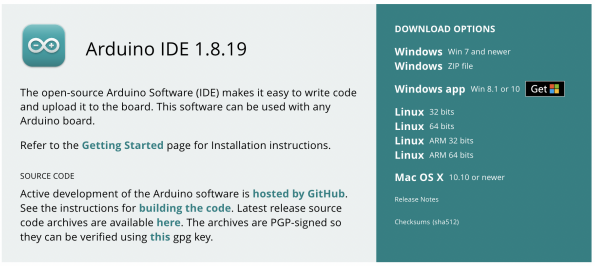
\includegraphics[width=1.0\textwidth]{Images/Deployment/Arduino-Nano-website-downloads-page}
	\caption{Arduino Nano website downloads page} \label{fig:Arduino-Nano-website-downloads-page}
\end{figure}

In order to carry out the project offline, the software should be downloaded in to the
desktop. The latest version of the software is preferred to be downloaded as it contains
all the performance improvements and bug fixes.The software can be installed in to
multiple operating systems like Windows, Mac OS and Linux. For this project version
1.8.19 was downloaded. After installation the libraries has to be configured for the
Arduino Nano BLE 33 sense board to work which is explained in the next section.

\begin{figure}[h!]
	\centering
	
\includegraphics[width=1.0\textwidth]{Images/Deployment/Arduino-Nano-software-version-number}
	\caption{Arduino Nano software version number} \label{fig:Arduino-Nano-software-version-number}
\end{figure}


\textbf{Configuration}

After installation of Arduino IDE, a window as is shown in figure \ref{fig:Arduino-IDE-initial-software-window}

In this project an Arduino Nano BLE 33 sense is used, that specific board has to be installed. This done by toggling through option navigating to Tools - > Boards - > Boards Manager as shown in the figure \ref{fig:Arduino-IDE-Boards-Manager-menu}

On opening the boards manager, a search bar is present that lets you to search, download and install the necessary libraries. A compatible board has to be downloaded and installed for the hardware to work properly. In this scenario, an Arduino Nano
mbed OS nano board has to be downloaded and installed as shown in figure \ref{fig:Arduino-IDE-Boards-Manager-list}

After installing the boards, the board has to be selected from the menu as shown in figure \ref{fig:Selection-of-correct-board-for-the-program}. For the keyword spotting project, Arduino Nano 33 BLE has to be selected as the board.

Connect the board to a computer using a USB cable and select the correct port from the menu by going to Tools -> Port -> Arduino Nano BLE 33 as shown in figure \ref{fig:Selection-of-correct-port-for-uploading-the-program} .
If the board is not seen in the drop down menu, ensure that the board libraries are downloaded and installed.

In order to confirm the board is connected and to check the details of the connected board, navigate to Tools -> Get Board Info where a window is produced as shown in
figure \ref{fig:Arduino-Board-Info}

For the Arduino Nano BLE 33 sense to work necessary libraries has to be installed in order to function properly. This can be done my navigating through Tools -> Manage Libraries as shown in figure \ref{fig:Managing-libraries-in-the-Arduino-IDE}. Search for Tensor flow libraries and then download and install them.

\begin{figure}[h!]
	\centering
	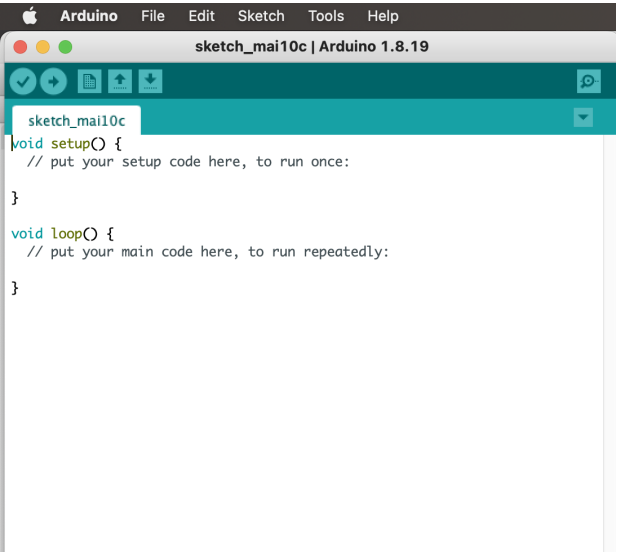
\includegraphics[width=1.0\textwidth]{Images/Deployment/Arduino-IDE-initial-software-window}
	\caption{Arduino IDE initial software window} \label{fig:Arduino-IDE-initial-software-window}
\end{figure}

\begin{figure}[h!]
	\centering
	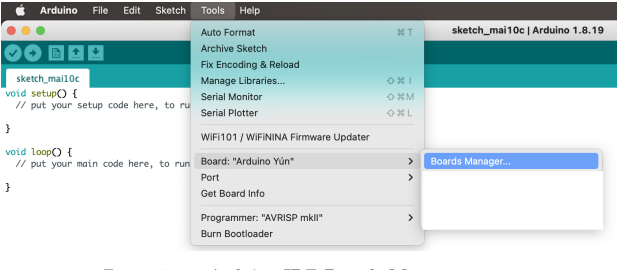
\includegraphics[width=1.0\textwidth]{Images/Deployment/Arduino-IDE-Boards-Manager-menu}
	\caption{Arduino IDE Boards Manager menu} \label{fig:Arduino-IDE-Boards-Manager-menu}
\end{figure}

\begin{figure}[h!]
	\centering
	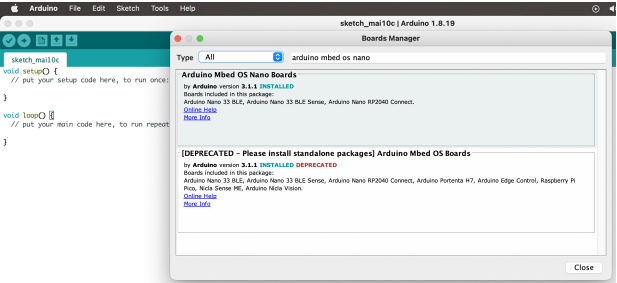
\includegraphics[width=1.0\textwidth]{Images/Deployment/Arduino-IDE-Boards-Manager-list}
	\caption{Arduino IDE Boards Manager list} \label{fig:Arduino-IDE-Boards-Manager-list}
\end{figure}

\begin{figure}[h!]
	\centering
	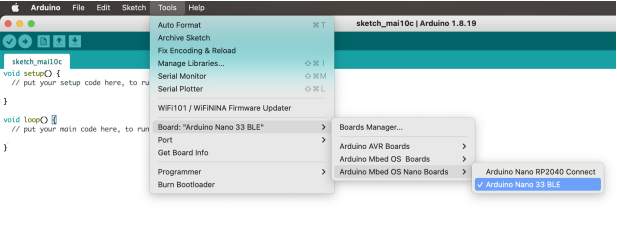
\includegraphics[width=1.0\textwidth]{Images/Deployment/Selection-of-correct-board-for-the-program}
	\caption{Selection of correct board for the program} 
	\label{fig:Selection-of-correct-board-for-the-program}
\end{figure}

\begin{figure}[h!]
	\centering
	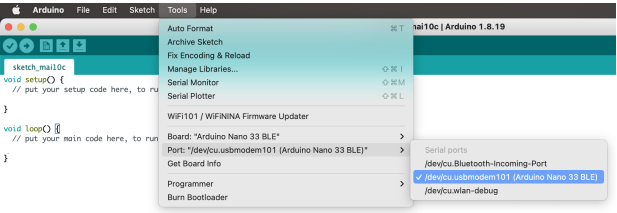
\includegraphics[width=1.0\textwidth]{Images/Deployment/Selection-of-correct-port-for-uploading-the-program}
	\caption{Selection of correct port for uploading the program} 
	\label{fig:Selection-of-correct-port-for-uploading-the-program}
\end{figure}

\begin{figure}[h!]
	\centering
	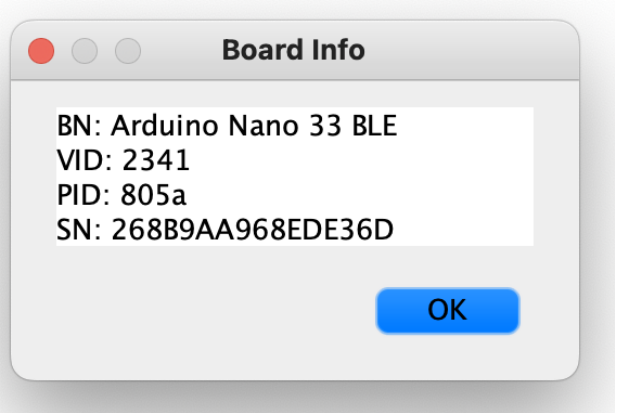
\includegraphics[width=1.0\textwidth]{Images/Deployment/Arduino-Board-Info}
	\caption{Arduino Board Info} 
	\label{fig:Arduino-Board-Info}
\end{figure}

\begin{figure}[h!]
	\centering
	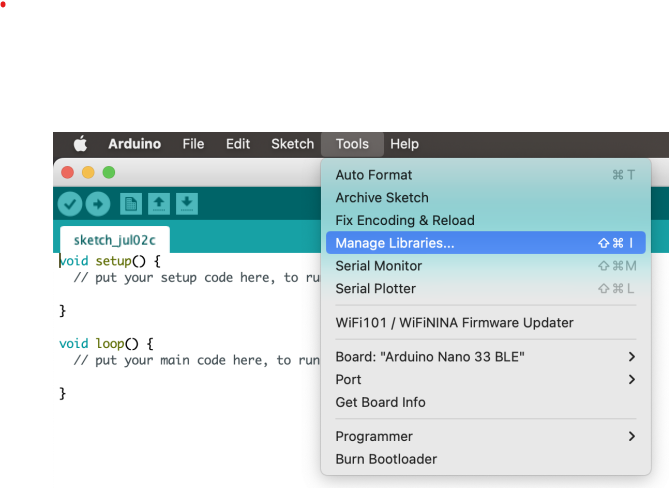
\includegraphics[width=1.0\textwidth]{Images/Deployment/Managing-libraries-in-the-Arduino-IDE}
	\caption{Managing libraries in the Arduino IDE} 
	\label{fig:Managing-libraries-in-the-Arduino-IDE}
\end{figure}



\subsection{Connecting an Arduino Nano 33 BLE Sense to a computer}

\textbf{Requirements:}

\begin{enumerate}
	\item Arduino Nano 33 BLE Sense.
	\item USB Cable.
	\item Arduino IDE.
\end{enumerate}

\textbf{Steps:}

\begin{enumerate}
	\item Install Arduino IDE Drivers:
	\begin{itemize}
		\item Open the Arduino IDE.
		\item Go to "Tools" > "Board" > "Boards Manager."
		\item Search for "Arduino mbed-enabled Boards" and install it.
	\end{itemize}
	\item Select Arduino Nano 33 BLE Sense:
	\begin{itemize}
		\item In the Arduino IDE, go to "Tools" > "Board" and select "Arduino Mbed OS Boards" > "Arduino Nano 33 BLE."
	\end{itemize}
	\item Install USB Driver
	\begin{itemize}
		\item For Windows users, you might need to install additional drivers. Follow the instructions provided on the Arduino website for Windows drivers.
	\end{itemize}
	\item Connect Arduino to Computer:
	\begin{itemize}
		\item Connect the Arduino Nano 33 BLE Sense to your computer using the USB cable.
	\end{itemize}
	\item Select Port:
	\begin{itemize}
         \item In the Arduino IDE, go to "Tools" > "Port" and select the port to which the Arduino Nano is connected. The port might look like COMx (Windows) or /dev/ttyUSBx (Linux) or /dev/cu.usbmodemxxxx (macOS).
     \end{itemize}
     \item Upload a Test Sketch:
     \begin{itemize}
     	\item Open an example sketch to test the connection. For example, go to "File" > "Examples" > "01.Basics" > "Blink."
     	\item Click the "Upload" button (right arrow icon) to upload the sketch to the Arduino. You should see the built-in LED on the Nano 33 BLE Sense blink.
     \end{itemize}
 \end{enumerate}         





\subsection{Install the TensorFlow Lite runtime}
In this project, all you need from the TensorFlow Lite API is the Interpreter class. So instead of installing the large tensorflow package, we're using the much smaller \texttt{tflite\_runtime} package.
To install this on your Arduino, follow the instructions in the Python quick start.

You can install the TFLite runtime using this script.

\begin{verbatim}
	sh setup.sh
\end{verbatim}

\section{TensorFlow Lite}
TensorFlow Lite is a mobile library for deploying machine learning models on mobile, microcontrollers, and other edge devices \url{https://www.tensorflow.org/lite/api_docs}. It is a solution for running machine learning models on mobile devices where luxuries such as huge disk space and GPUs are not usable. TensorFlow Lite is specially optimized for on-device machine learning (Edge ML). It supports platforms such as embedded Linux, Android, iOS, and MCU. TensorFlow Lite takes existing models and converts them into an optimized version within the sort of .tflite file. The new file format supported by TensorFlow Lite is Flat Buffers.

The TensorFlow Lite library provides a set of tools that enables on-device machine learning by allowing developers to run their trained models on mobile, embedded, and IoT devices and computers. It allows one to execute machine learning models easily on a smartphone, allowing one to perform traditional machine learning tasks without the need for an external API or server. In contrast to server-based architectures, TensorFlow Lite is a more effective alternative to mobile model enablement. On mobile devices, it allows offline inference.

TensorFlow Lite is used to develop TensorFlow models and integrate that model into a mobile environment\cite{Boesch:2021}. It is also used to recognize speech keywords "yes" and "no" using the Arduino Nano 33 BLE Sensor. The TensorFlow Lite Micro Library is used to preprocess the audio data and recognize the speech keywords.

Please note that TensorFlow Lite does not optimize model size, so mobile devices may require larger storage. In the TensorFlow Lite process, the expense of reliability and optimization is a trade-off with the model’s accuracy. As a result, TensorFlow Lite models are less accurate than their full-featured counterparts.

\subsection{Code Example}
To recognize speech keywords "yes" and "no" using the Arduino Nano 33 BLE Sensor, you can use the TensorFlow Lite Micro Library \cite{Arduino:2023}.Here is a sample code in Python that you can use as a starting point:

\begin{code}[h!]
	\lstinputlisting[language=Python, numbers=none, linerange={1-100}]{Code/Deployment/TensorflowLiteSampleCode.py}    
	
	\caption{Sample code}
	\label{code:sampleCode}
\end{code}

This code uses the micro\_speech library to record audio from the microphone and preprocess it for the TensorFlow Lite model. The model is loaded from the file, which should be trained to recognize the speech keywords "yes" and "no". The recognized keyword is printed to the console.

Please note that this is just a sample code and you will need to modify it to suit your specific requirements. You may also need to install additional libraries and dependencies to run this code on your system. Please refer to the given sample code \ref{code:sampleCode}


\subsection{Use in the project}
Creating a speech keyword recognition model and deploying it on Arduino Nano 33 BLE Sense involves several steps. Due to the resource constraints of the Arduino Nano, we'll use a simple machine learning model. One popular approach for this task is to use MFCC features with a machine learning classifier like Support Vector Machine (SVM).
Here's the Python code for our model:

Please refer to the given code - (see Listing \ref{code:DeployableCode}).

Please refer to the given code - (see Listing \ref{code:DeployableCodeII}).

\textbf{LED control:}

Based on the recognized command, control the onboard LEDs accordingly
\begin{itemize}
	\item For "yes" command: Illuminate the green LED.
	\item For "no" command: Illuminate the red LED.
	\item For unrecognized keyword the blue LED would be turned on.
\end{itemize} 

\section{TensorFlow Lite Micro}
TensorFlow Lite Micro is a framework that provides a set of tools for running neural network inference on microcontrollers \url{https://www.tensorflow.org/lite/api_docs}. It is designed to run machine learning models on microcontrollers and other devices with only a few kilobytes of memory. The core runtime just fits in 16 KB on an Arm Cortex M3 and can run many basic models. It doesn’t require operating system support, any standard C or C++ libraries, or dynamic memory allocation.

TensorFlow Lite Micro is a solution for running machine learning models on mobile devices where luxuries such as huge disk space and GPUs are not usable. It is specially optimized for on-device machine learning (Edge ML) 2. It supports platforms such as embedded Linux, Android, iOS, and MCU 2. TensorFlow Lite Micro takes existing models and converts them into an optimized version within the sort of .tflite file. The new file format supported by TensorFlow Lite Micro is Flat Buffers.

The TensorFlow Lite Micro library provides a set of tools that enables on-device machine learning by allowing developers to run their trained models on mobile, embedded, and IoT devices and computers 2. It allows one to execute machine learning models easily on a smartphone, allowing one to perform traditional machine learning tasks without the need for an external API or server \url{https://www.tensorflow.org/lite/api_docs}. In contrast to server-based architectures, TensorFlow Lite Micro is a more effective alternative to mobile model enablement. On mobile devices, it allows offline inference.

TensorFlow Lite Micro is used to develop TensorFlow models and integrate that model into a mobile environment 2. It is also used to recognize speech keywords "yes" and "no" using the Arduino Nano 33 BLE Sensor. The TensorFlow Lite Micro Library is used to preprocess the audio data and recognize the speech keywords.

Please note that TensorFlow Lite Micro is limited to model inference and does not support training 2. It is also important to note that TensorFlow Lite does not optimize model size, so mobile devices may require larger storage. In the TensorFlow Lite process, the expense of reliability and optimization is a trade-off with the model’s accuracy. As a result, TensorFlow Lite models are less accurate than their full-featured counterparts.

\begin{code}[h!]
	\lstinputlisting[language=Python, numbers=none, linerange={1-50}]{Code/Deployment/DeployableCode.py}    
	\caption{Deployable Code Part-I}
	\label{code:DeployableCode}
\end{code}
\begin{code}[h!]
	\lstinputlisting[language=Python, numbers=none, linerange={51-88}]{Code/Deployment/DeployableCode.py}    
	\caption{Deployable Code Part-II }
	\label{code:DeployableCodeII}
\end{code}